\documentclass[11pt]{amsart}
\usepackage{amsmath,amssymb,amsthm,graphicx,booktabs,xcolor}
\usepackage[margin=1.1in]{geometry}
\usepackage[colorlinks=true,linkcolor=blue!50!black,citecolor=blue!50!black,urlcolor=blue!50!black]{hyperref}

\newtheorem{theorem}{Theorem}
\newtheorem{proposition}[theorem]{Proposition}
\newtheorem{lemma}[theorem]{Lemma}
\theoremstyle{remark}
\newtheorem{remark}[theorem]{Remark}

\newcommand{\eps}{\varepsilon}
\newcommand{\e}{\mathrm{e}}
\newcommand{\cX}{\mathcal{X}}
\newcommand{\cB}{\mathcal{B}}
\newcommand{\ov}{\overline}
\newcommand{\Tr}{\operatorname{Tr}}
\newcommand{\SL}{\mathrm{SL}_2(\mathbb Z)}

\title{Murmurations of modular forms with nebentypus}
\author{Ramanuja}
\address{Madhubani, Bihar, India}
\date{\today}

\begin{document}

\begin{abstract}
We study murmurations in the simplest family of modular forms that are not self-dual: newforms of weight $k\ge2$ and odd squarefree level $N$ whose nebentypus is a primitive character modulo $N$. For these forms the root number $\eps_f$ is a complex number of modulus one. We show that, after averaging over the characters, it correlates with the Hecke eigenvalues $\ov{\lambda_f(p)}$ of the dual form, and that the correlation is a single Bessel function. With harmonic weights the average of $\eps_f\ov{\lambda_f(p)}$ is $\frac{2\pi}{\sqrt N}J_{k-1}(4\pi\sqrt{p/N})$ up to a smaller error. With natural weights it is $\frac{2\pi}{\zeta^{(N)}(2)\sqrt N}(1+\frac1p)J_{k-1}(4\pi\sqrt{p/N})$, where $\zeta^{(N)}(2)$ omits the Euler factors at the primes dividing $N$. Both results are unconditional and hold for each individual level, with no average over $N$. By contrast, the average of $\eps_f\lambda_f(p)$ is negligible unless $p$ lies in a few special residue classes modulo $N$. The harmonic results follow from the Petersson formula, where the whole main term comes from the first Kloosterman modulus. For the natural results we expand a twisted sum of Hurwitz class numbers in Chebyshev polynomials and interpret every mode as a trace of a Hecke operator; only the Eisenstein contribution survives. Numerical computations with the exact trace formula, for levels up to $900$ and weights $2\le k\le6$, confirm both the main terms and the sizes of the errors.
\end{abstract}

\maketitle

\section{Introduction}

\subsection{Background}
Murmurations are correlations between root numbers and Hecke eigenvalues at primes whose size is comparable to the conductor. He, Lee, Oliver and Pozdnyakov discovered them for elliptic curves \cite{HLOP}, and Zubrilina gave the first proof, for holomorphic newforms of fixed weight, trivial character and squarefree level \cite{Zub}. Murmurations have since been established in the weight aspect \cite{BBLLD,KL}, for Maass forms \cite{BLLDSHZ}, in the depth aspect \cite{Tom}, for Dirichlet characters \cite{LOP}, and, conditionally on ratios conjectures, for further families \cite{Cow}; see also \cite{LD,Car}. In all holomorphic families treated so far the forms are self-dual, so that $\eps_f=\pm1$.

This paper treats families that are not self-dual. Here the root number is a complex number of modulus one, and it is not clear a priori what it should correlate with. We show that the answer is the Hecke eigenvalue of the \emph{dual} form, and that the resulting murmuration density is a single Bessel function, at every individual level.

\subsection{Setup}
Fix an integer $k\ge2$ and a prime $q$ (the case of odd squarefree level is treated in Section~\ref{sec:composite}). Let
\[
\cX_k(q)=\{\chi \bmod q:\ \chi\ne\chi_0,\ \chi(-1)=(-1)^k\},\qquad |\cX_k(q)|=\tfrac{q-1}{2}-\delta_{2\mid k}.
\]
Every $\chi\in\cX_k(q)$ is primitive, so $S_k(q,\chi)$ has no oldforms; let $\cB_k(q,\chi)$ be its basis of normalized newforms. For $f\in\cB_k(q,\chi)$ write $a_f(n)=\lambda_f(n)\,n^{(k-1)/2}$ for its Fourier coefficients and $\bar f(z)=\ov{f(-\bar z)}\in S_k(q,\bar\chi)$ for its dual. The root number $\eps_f$ is defined by
\[
\Lambda(f,s)=\eps_f\,\Lambda(\bar f,k-s),\qquad \Lambda(f,s)=\Bigl(\tfrac{\sqrt q}{2\pi}\Bigr)^s\Gamma(s)L(f,s).
\]
With the harmonic weights $\omega_f=\Gamma(k-1)(4\pi)^{1-k}\|f\|^{-2}$ we define two averages over the family:
\[
\langle \alpha\rangle_h=\frac{1}{|\cX_k(q)|}\sum_{\chi\in\cX_k(q)}\ \sum_{f\in\cB_k(q,\chi)}\omega_f\,\alpha(f),\qquad
\langle \alpha\rangle=\frac{\sum_{\chi}\sum_{f}\alpha(f)}{\sum_\chi \dim S_k(q,\chi)}.
\]
Throughout, $\e(x)=\exp(2\pi ix)$, $\tau(\chi)=\sum_{x\bmod q}\chi(x)\e(x/q)$ is the Gauss sum, $\sigma_0(n)$ is the number of divisors of $n$, and $J_{k-1}$ is the Bessel function of the first kind.

\subsection{Results at prime level}
Our first result concerns the harmonic average.

\begin{theorem}\label{thm:main}
Let $k\ge2$, let $q$ be prime and let $p\neq q$ be a prime with $p\le q^2$. Then
\[
\bigl\langle \eps_f\,\ov{\lambda_f(p)}\bigr\rangle_h=\frac{2\pi}{\sqrt q}\,J_{k-1}\!\Bigl(4\pi\sqrt{\tfrac pq}\Bigr)+O_{k,\varepsilon}\!\Bigl(q^{-1+\varepsilon}\bigl(1+\tfrac pq\bigr)^{1/4+\varepsilon}\Bigr).
\]
\end{theorem}

Since $J_{k-1}(x)$ oscillates with amplitude $\asymp x^{-1/2}$, the main term has size $q^{-1/2}(p/q)^{-1/4}$ and dominates the error for $p\le q^{2-\delta}$. In the proof, the entire main term comes from the first Kloosterman modulus $c=q$ in the Petersson formula: there the Gauss sums cancel exactly, and the contribution is the same for every character. The other moduli are made small by the average over $\chi$.

The conjugation in Theorem~\ref{thm:main} is essential. Without it the correlation disappears, except for special primes.

\begin{theorem}\label{thm:unconj}
Under the hypotheses of Theorem~\ref{thm:main}, let $c_k(p,q)=|\cX_k(q)|^{-1}\sum_{\chi\in\cX_k(q)}\chi(p)$, so that
\[
c_k(p,q)=\frac{q-1}{2|\cX_k(q)|}\bigl(\mathbf 1_{p\equiv1\,(q)}+(-1)^k\mathbf 1_{p\equiv-1\,(q)}\bigr)-\frac{\delta_{2\mid k}}{|\cX_k(q)|}.
\]
Then
\begin{multline*}
\bigl\langle \eps_f\,\lambda_f(p)\bigr\rangle_h=c_k(p,q)\,\frac{2\pi}{\sqrt q}J_{k-1}\!\Bigl(4\pi\sqrt{\tfrac pq}\Bigr)\\
+O\Bigl(q^{-1+\varepsilon}\bigl(1+\tfrac pq\bigr)^{1/4+\varepsilon}+q^{-1/2+\varepsilon}\!\!\sum_{\substack{r\ge2\\ r\equiv\pm p\,(q)}}\!\frac{|J_{k-1}(4\pi\sqrt{p/q}/r)|}{\sqrt r}\Bigr).
\end{multline*}
In particular, for $p/q$ in a fixed compact set, $\langle\eps_f\lambda_f(p)\rangle_h=o(q^{-1/2})$ unless $p\equiv\pm1\pmod q$ or the least positive residue of $\pm p$ modulo $q$ is bounded.
\end{theorem}

This is what the approximate functional equation suggests: there $\eps_f$ multiplies the Dirichlet series $\sum_n\ov{\lambda_f(n)}n^{-s}$ of $\bar f$, not that of $f$.

For the natural average we do not remove the harmonic weights. Instead we work directly with the Eichler--Selberg trace formula and obtain a sharper error term.

\begin{theorem}\label{thm:natural}
Let $k\ge2$, let $q$ be prime and let $p\ne q$ be prime. Then
\[
\bigl\langle \eps_f\,\ov{\lambda_f(p)}\bigr\rangle=\frac{12}{\pi\sqrt q}\Bigl(1+\frac1p\Bigr)J_{k-1}\!\Bigl(4\pi\sqrt{\tfrac pq}\Bigr)+O_{k,\varepsilon}\Bigl(q^{-3/2+\varepsilon}\bigl(1+\tfrac pq\bigr)\Bigr).
\]
\end{theorem}

The main term dominates for $p\le q^{9/5-\delta}$. Since $12/\pi=2\pi/\zeta(2)$, the natural density is $1/\zeta(2)$ times the harmonic one; Remark~\ref{rem:zeta2} explains this factor from the Petersson side. The proof (Section~\ref{sec:natural}) starts from an exact formula for the natural average in terms of Hurwitz class numbers $H(\cdot)$ (Proposition~\ref{prop:exact}). After the average over $\chi$, the Gauss sums produce the additive character $\e(t/q)$. Since $t$ ranges over $|t|<2\sqrt{pq}$, this character is a smooth function of $u=t/2\sqrt{pq}$, namely $\exp(4\pi i\sqrt{p/q}\,u)$. We expand it in the Chebyshev polynomials $U_m$, which turns the problem into the untwisted sums $\sum_tU_m(t/2\sqrt n)H(4n-t^2)$. For $m\ge2$ these are traces of $T_n$ on $S_{m+2}(\SL)$, hence $O(\sqrt n)$ by Deligne's bound. For $m=0$ the Kronecker--Hurwitz relation gives $2\sigma(n)+O(\sqrt n)$. That single term produces the Bessel function and the constant $12/\pi$.

\subsection{Results at squarefree level}
For odd squarefree $N$ and the family of primitive characters modulo $N$, Theorem~\ref{thm:main} carries over unchanged (Theorem~\ref{thm:compositeh}). For the natural average the constant changes: it becomes $2\pi/\zeta^{(N)}(2)$ with $\zeta^{(N)}(2)=\zeta(2)\prod_{\ell\mid N}(1-\ell^{-2})$ (Theorem~\ref{thm:compositenat}). The proof of Theorem~\ref{thm:natural} does not apply directly. Besides $\e(t/N)$, the character sum now contains twists that are periodic modulo each prime $\ell\mid N$. We expand these into multiplicative characters $\psi\bmod N$. Every resulting class number sum is then a trace of $T_{pN}$ on some space $S_K(N,\psi)$, and these traces are small. The main term comes from the Eisenstein contribution to the weight-two trace for the principal character.

\subsection{Comparison with the self-dual case}
Zubrilina's density for trivial character is an explicit arithmetic sum, and murmurations in self-dual families are usually established after an additional average over levels. In the family studied here the average over characters plays that role. It produces a density with a single Bessel term, and it does so at every individual level.

\subsection*{Organization}
Section~\ref{sec:prelim} collects the root number formula, the Petersson formula and a character sum identity. Section~\ref{sec:harmonic} proves Theorems~\ref{thm:main} and~\ref{thm:unconj}. Section~\ref{sec:natural} proves Theorem~\ref{thm:natural} and reports numerical tests. Section~\ref{sec:composite} treats squarefree level, and Section~\ref{sec:questions} lists open questions. The code that produces all tables and figures is available at \url{https://github.com/ramanujamath/nebentypus-murmurations}.

\section{Preliminaries}\label{sec:prelim}

\subsection{Root numbers}
Let $W_q$ act by $(f|_kW_q)(z)=q^{k/2}(qz)^{-k}f(-1/(qz))$; it maps $S_k(q,\chi)$ to $S_k(q,\bar\chi)$. Taking the Mellin transform of $f(iy)$ and substituting $y\mapsto1/(qy)$ gives
\begin{equation}\label{eq:FE}
\Lambda(f,s)=i^k\,\Lambda(f|_kW_q,\,k-s).
\end{equation}
For a newform $f$ we have $f|_kW_q=\eta_f\,\bar f$ with a pseudo-eigenvalue $\eta_f$ of modulus one. By Atkin--Li \cite[Thm.~2.1]{AL}, with our normalization of $W_q$,
\begin{equation}\label{eq:AL}
\eta_f=\chi(-1)\,\frac{\tau(\chi)\,q^{k/2-1}}{a_f(q)},\qquad |a_f(q)|=q^{(k-1)/2}.
\end{equation}
Since $\chi(-1)=(-1)^k$ and $\eps_f=i^k\eta_f$ by \eqref{eq:FE}, we obtain the following lemma.

\begin{lemma}\label{lem:root}
For $f\in\cB_k(q,\chi)$, $\displaystyle \eps_f=i^{-k}\,\frac{\tau(\chi)}{\sqrt q}\,\ov{\lambda_f(q)}$.
\end{lemma}

\begin{remark}
Conventions for $W_q$ differ in the literature, and a wrong sign would change the main terms below. We therefore verified Lemma~\ref{lem:root} numerically. For every one-dimensional space $S_k(q,\chi)$ with $(q,k)\in\{(11,3),(13,2),(17,2),(7,4),(5,5)\}$, we computed $f$ from Hecke traces and evaluated $f|_kW_q/\bar f$ at generic points; the result always agreed with \eqref{eq:AL}.
\end{remark}

For $p\ne q$ we also use $\ov{a_f(p)}=\bar\chi(p)\,a_f(p)$, that is, $\ov{\lambda_f(p)}=\bar\chi(p)\lambda_f(p)$.

\subsection{The Petersson formula}
For $m,n\ge1$ and $q\mid c$ let $S_\chi(m,n;c)=\sum_{d\bmod c}^{*}\chi(d)\,\e\bigl((m\bar d+nd)/c\bigr)$. Then \cite[Prop.~14.5]{IK}
\begin{equation}\label{eq:pet}
\sum_{f\in\cB_k(q,\chi)}\omega_f\,\lambda_f(m)\ov{\lambda_f(n)}=\delta_{m,n}+2\pi i^{-k}\sum_{r\ge1}\frac{S_\chi(m,n;qr)}{qr}\,J_{k-1}\!\Bigl(\frac{4\pi\sqrt{mn}}{qr}\Bigr).
\end{equation}
Which argument carries $\chi$, and which side carries the complex conjugation, matters for our main terms. We confirmed \eqref{eq:pet} as stated numerically for $q=11$, $k=3$: we summed the right-hand side over $c\le11\cdot1500$ and compared it with $\lambda_f(m)\ov{\lambda_f(n)}$ in the one-dimensional spaces.

\subsection{A character sum}
\begin{lemma}\label{lem:charsum}
For $(a,q)=1$,
\[
\sum_{\chi\in\cX_k(q)}\tau(\chi)\chi(a)=\frac{q-1}{2}\Bigl(\e\bigl(\tfrac{\bar a}{q}\bigr)+(-1)^k\e\bigl(-\tfrac{\bar a}{q}\bigr)\Bigr)+\delta_{2\mid k}.
\]
\end{lemma}
\begin{proof}
Expand $\tau(\chi)$ and use orthogonality in the form
\[
\sum_{\chi(-1)=(-1)^k}\chi(m)=\tfrac{q-1}{2}\bigl(\mathbf 1_{m\equiv1}+(-1)^k\mathbf 1_{m\equiv-1}\bigr).
\] When $k$ is even, the trivial character must be removed; its Gauss sum is $\sum_{x\not\equiv0}\e(x/q)=-1$.
\end{proof}

We also use Weil's bound $|S(m,n;c)|\le\sigma_0(c)\,(m,n,c)^{1/2}c^{1/2}$ for the classical Kloosterman sum $S(m,n;c)$, and the bound $|J_{k-1}(x)|\le\min\bigl(1,(x/2)^{k-1}/(k-1)!\bigr)$.

\section{Harmonic weights: proofs of Theorems \ref{thm:main} and \ref{thm:unconj}}\label{sec:harmonic}

\begin{proof}[Proof of Theorem \ref{thm:main}]
By Lemma~\ref{lem:root} and $\ov{\lambda_f(p)}=\bar\chi(p)\lambda_f(p)$,
\[
\sum_{f}\omega_f\,\eps_f\ov{\lambda_f(p)}=i^{-k}\,\frac{\tau(\chi)\bar\chi(p)}{\sqrt q}\sum_f\omega_f\,\lambda_f(p)\ov{\lambda_f(q)}.
\]
We apply \eqref{eq:pet} with $(m,n)=(p,q)$. The diagonal term vanishes. Put $x=4\pi\sqrt{p/q}$.

\emph{The modulus $c=q$.} Here $S_\chi(p,q;q)=\sum_d\chi(d)\e(p\bar d/q)=\chi(p)\tau(\bar\chi)$, and $\tau(\chi)\tau(\bar\chi)=\chi(-1)q=(-1)^kq$. The contribution is therefore
\[
i^{-2k}\,\frac{\tau(\chi)\bar\chi(p)}{\sqrt q}\cdot 2\pi\,\frac{\chi(p)\tau(\bar\chi)}{q}\,J_{k-1}(x)=\frac{2\pi}{\sqrt q}J_{k-1}(x).
\]
It is the same for every $\chi$, so it survives the average over $\chi$ and gives the main term.

\emph{The moduli $c=qr$ with $r\ge2$.} By Lemma~\ref{lem:charsum} with $a=d\bar p$, and since $\e(p\bar d/q)=\e(pr\bar d/(qr))$,
\[
\sum_{\chi\in\cX_k(q)}\tau(\chi)\bar\chi(p)S_\chi(p,q;qr)=\frac{q-1}{2}\Bigl(S\bigl(p(1+r),q;qr\bigr)+(-1)^kS\bigl(p(1-r),q;qr\bigr)\Bigr)+\delta_{2\mid k}S(p,q;qr).
\]
As $p\ne q$, the gcd $(p(1\pm r),q,qr)$ equals $q$ if $r\equiv\mp1\pmod q$ and $1$ otherwise. By Weil's bound, the moduli $c=qr$ with $r\ge2$ contribute to $\langle\eps_f\ov{\lambda_f(p)}\rangle_h$ at most
\[
\ll q^{-1/2}\sum_{r\ge2}\frac{\sigma_0(qr)(qr)^{1/2}}{qr}\,|J_{k-1}(x/r)|\Bigl(1+q^{1/2}\,\mathbf 1_{r\equiv\pm1\,(q)}\Bigr).
\]
For $r\not\equiv\pm1$ we split at $r=x$ and use $|J_{k-1}(x/r)|\le\min(1,(x/r)^{k-1})$. Since $k\ge2$, these terms give
\[
\ll q^{-1+\varepsilon}\Bigl(\sum_{r\le x}r^{-1/2+\varepsilon}+\sum_{r>x}r^{-1/2+\varepsilon}(x/r)^{k-1}\Bigr)\ll q^{-1+\varepsilon}(1+x)^{1/2+2\varepsilon}.
\]
For $r\equiv\pm1$ we have $r\ge q-1$, and $x\ll q^{1/2}$ because $p\le q^2$. These terms give
\[
\ll q^{-1/2+\varepsilon}x^{k-1}\sum_{\substack{r\ge q-1\\ r\equiv\pm1\,(q)}}r^{-k+1/2+\varepsilon}\ll q^{-k+\varepsilon}x^{k-1}\ll q^{-(k+1)/2+\varepsilon},
\]
which is admissible. Since $(1+x)^{1/2}\asymp(1+p/q)^{1/4}$, the theorem follows.
\end{proof}

\begin{proof}[Proof of Theorem \ref{thm:unconj}]
Now $\sum_f\omega_f\eps_f\lambda_f(p)=i^{-k}q^{-1/2}\tau(\chi)\sum_f\omega_f\lambda_f(p)\ov{\lambda_f(q)}$, without the factor $\bar\chi(p)$. The modulus $c=q$ therefore contributes $\frac{2\pi}{\sqrt q}\chi(p)J_{k-1}(x)$, and averaging over $\chi$ produces $c_k(p,q)$. For $r\ge2$, Lemma~\ref{lem:charsum} with $a=d$ gives
\[
\sum_{\chi\in\cX_k(q)}\tau(\chi)S_\chi(p,q;qr)=\frac{q-1}{2}\Bigl(S(p+r,q;qr)+(-1)^kS(p-r,q;qr)\Bigr)+\delta_{2\mid k}S(p,q;qr).
\]
The gcd $(p\pm r,q)$ equals $q$ exactly when $r\equiv\mp p\pmod q$. The estimate proceeds as before; the exceptional values of $r$ produce the last error term.
\end{proof}

\section{Natural weights: proof of Theorem \ref{thm:natural}}\label{sec:natural}

\subsection{An exact formula}
By Lemma~\ref{lem:root} and multiplicativity, $\eps_f\ov{\lambda_f(p)}=i^{-k}q^{-1/2}\tau(\chi)\,\ov{\lambda_f(pq)}=i^{-k}q^{-1/2}\tau(\chi)\,\lambda_{\bar f}(pq)$. Since $f\mapsto\bar f$ is a bijection from $\cB_k(q,\chi)$ to $\cB_k(q,\bar\chi)$,
\[
\sum_{f\in\cB_k(q,\chi)}\eps_f\ov{\lambda_f(p)}=\frac{i^{-k}\tau(\chi)}{\sqrt q\,(pq)^{(k-1)/2}}\Tr\bigl(T_{pq}\mid S_k(q,\bar\chi)\bigr).
\]
We evaluate the trace with the Eichler--Selberg trace formula for $S_k(\Gamma_0(N),\chi)$ \cite[Thm.~12.4.11]{CS}. Write $P_k(t,n)=(\rho^{k-1}-\bar\rho^{k-1})/(\rho-\bar\rho)$, where $\rho+\bar\rho=t$ and $\rho\bar\rho=n$, and let $H$ be the Hurwitz class number. For $n=pq$ the elliptic terms simplify. If $s^2\mid t^2-4pq$, then $q\nmid s$, since $q\mid s$ would force $q\mid t$ and then $q^2\mid4pq$. Moreover $x^2-tx+pq\equiv x(x-t)\pmod q$, so the local factor at $q$ is $\bar\chi(0)+\bar\chi(t)=\bar\chi(t)$. The hyperbolic terms can be computed directly. Altogether,
\[
\Tr\bigl(T_{pq}\mid S_k(q,\bar\chi)\bigr)=-\tfrac12\sum_{t^2<4pq}P_k(t,pq)\,\bar\chi(t)\,H(4pq-t^2)-1-\bar\chi(p)\min(p,q)^{k-1}.
\]
Summing over $\chi$ with Lemma~\ref{lem:charsum} yields the following exact formula.

\begin{proposition}\label{prop:exact}
Let $G_k(b)=q^{-1/2}\bigl[\frac{q-1}{2}\bigl(\e(b/q)+(-1)^k\e(-b/q)\bigr)+\delta_{2\mid k}\bigr]$. Then
\[
\sum_{\chi\in\cX_k(q)}\sum_f\eps_f\ov{\lambda_f(p)}=\frac{i^{-k}}{(pq)^{\frac{k-1}{2}}}\Bigl[-\tfrac12\!\!\sum_{\substack{t^2<4pq\\ q\nmid t}}\!\!P_k(t,pq)H(4pq-t^2)G_k(t)-G_k(1)-\min(p,q)^{k-1}G_k(p)\Bigr].
\]
\end{proposition}

We checked Proposition~\ref{prop:exact}, and the analogous formula for $\eps_f\lambda_f(p)$, against direct eigenform computations in the one-dimensional spaces listed above; the two sides agree to machine precision.

\subsection{Two lemmas}
Let $U_m$ denote the Chebyshev polynomials of the second kind. They are orthogonal for the weight $\sqrt{1-u^2}$ on $[-1,1]$, with $\int_{-1}^1U_m^2\sqrt{1-u^2}\,du=\pi/2$, and $P_K(t,n)=n^{(K-2)/2}U_{K-2}\bigl(t/2\sqrt n\bigr)$.

\begin{lemma}[Eichler--Selberg in level one]\label{lem:ES1}
Let $n\ge1$ be a non-square and let $K\ge2$ be even. Then
\[
\sum_{t^2<4n}P_K(t,n)H(4n-t^2)=-2\Tr\bigl(T_n\mid S_K(\SL)\bigr)-\sum_{d\mid n}\min(d,n/d)^{K-1}+2\sigma(n)\,\delta_{K=2}.
\]
In particular, if $n=pq$ with distinct primes $p,q$, then $\sum_tH(4n-t^2)=2\sigma(n)-2-2\min(p,q)$.
\end{lemma}
\begin{proof}
This is the trace formula \cite[Thm.~12.4.11]{CS} for $N=1$ and trivial character; the term for square $n$ is absent. For $K=2$ we have $S_2(\SL)=0$, and the identity is the Kronecker--Hurwitz class number relation.
\end{proof}

\begin{lemma}\label{lem:cheb}
Let $k\ge2$ and $a>0$, and put $W(u)=U_{k-2}(u)\exp(iau)$. Then $W=\sum_{m\ge0}c_mU_m$ uniformly on $[-1,1]$, where
\[
c_0=2\,i^{k-2}(k-1)\frac{J_{k-1}(a)}{a},\qquad \sum_{m\ge0}(m+2)|c_m|\ll_k(1+a)^2 .
\]
\end{lemma}
\begin{proof}
Gegenbauer's expansion of the plane wave \cite[\S11.5]{Wat}, with $C^{(1)}_j=U_j$, reads $\exp(iau)=\frac2a\sum_{j\ge0}i^j(j+1)J_{j+1}(a)U_j(u)$. It converges absolutely and uniformly because $|U_j|\le j+1$ and $|J_{j+1}(a)|\le\min\bigl(1,(a/2)^{j+1}/(j+1)!\bigr)$. Multiply by $U_{k-2}$ and use the Clebsch--Gordan rule $U_{k-2}U_j=\sum U_l$, where $l$ runs from $|j-k+2|$ to $j+k-2$ in steps of $2$. Only $j=k-2$ contributes to the coefficient of $U_0$, which gives $c_0$. Each $j$ contributes to at most $k-1$ coefficients $c_l$, all with $l\le j+k$, so $\sum(m+2)|c_m|\ll_k\sum_j(j+1)^2|J_{j+1}(a)|/a$. This is $\ll1$ for $a\le1$. For $a>1$, the terms with $j+1\le2a$ contribute $\ll a^2$, and the remaining terms are exponentially small.
\end{proof}

\subsection{Proof of Theorem \ref{thm:natural}}
Put $n=pq$, $y=p/q$, $a=4\pi\sqrt y$ and $u_t=t/2\sqrt n$, so that $\e(t/q)=\exp(iau_t)$. Let $S_\pm=\sum_{t^2<4n}P_k(t,n)H(4n-t^2)\e(\pm t/q)$. Since $P_k(-t,n)=(-1)^kP_k(t,n)$, we have $S_-=(-1)^kS_+$, and hence
\[
\sum_{t^2<4n}P_k(t,n)H(4n-t^2)G_k(t)=\frac{q-1}{\sqrt q}\,S_++\frac{\delta_{2\mid k}}{\sqrt q}\sum_{t^2<4n}P_k(t,n)H(4n-t^2).
\]

\emph{Evaluation of $S_+$.} By Lemma~\ref{lem:cheb}, $S_+=n^{(k-2)/2}\sum_mc_m\Sigma_m$ with $\Sigma_m=\sum_tU_m(u_t)H(4n-t^2)$. If $m$ is odd, then $\Sigma_m=0$ by the symmetry $t\mapsto-t$. If $m\ge2$ is even, Lemma~\ref{lem:ES1} with $K=m+2$ and Deligne's bound $|\Tr(T_n\mid S_K(\SL))|\le\dim S_K(\SL)\,\sigma_0(n)\,n^{(K-1)/2}$ give
\[
|\Sigma_m|=n^{-m/2}\Bigl|2\Tr\bigl(T_n\mid S_{m+2}(\SL)\bigr)+\sum_{d\mid n}\min(d,\tfrac nd)^{m+1}\Bigr|\le\tfrac{2(m+2)}{3}\sqrt n+2+2\sqrt n,
\]
using $\dim S_K(\SL)\le K/12$, $\sigma_0(n)=4$ and $\min(p,q)\le\sqrt n$. Finally $\Sigma_0=2\sigma(n)-2-2\min(p,q)$ by Lemma~\ref{lem:ES1}. Therefore
\[
S_+=n^{(k-2)/2}\Bigl(c_0\bigl(2\sigma(n)-2-2\min(p,q)\bigr)+O_k\bigl(\sqrt n\,(1+y)\bigr)\Bigr).
\]

\emph{The remaining terms.} The sum in Proposition~\ref{prop:exact} excludes the values $t\equiv0\pmod q$; there are at most $4\sqrt y+1$ of them. Each has $|P_k(t,n)|\le(k-1)n^{(k-2)/2}$, $H(4n-t^2)\ll_\varepsilon n^{1/2+\varepsilon}$ and $|G_k(t)|\le\sqrt q$, so together they contribute $\ll_{k,\varepsilon}\sqrt q\,n^{(k-1)/2+\varepsilon}(1+\sqrt y)$. By Lemma~\ref{lem:ES1} and Deligne's bound, $\sum_tP_k(t,n)H(4n-t^2)\ll_kn^{k/2}$, so the $\delta_{2\mid k}$ term, including its factor $q^{-1/2}$, is $\ll_kn^{(k-1)/2}\sqrt p$. The terms $G_k(1)$ and $\min(p,q)^{k-1}G_k(p)$ are $\ll\sqrt q\,n^{(k-1)/2}$.

\emph{Assembling.} Since $-\tfrac12\,i^{-k}\,i^{k-2}=\tfrac12$ and $a\sqrt n=4\pi p$, Proposition~\ref{prop:exact} becomes
\[
\sum_\chi\sum_f\eps_f\ov{\lambda_f(p)}=\frac{(q-1)(k-1)}{4\pi p\sqrt q}\bigl(2\sigma(n)-2-2\min(p,q)\bigr)J_{k-1}(a)+O_{k,\varepsilon}\bigl(q^{1/2+\varepsilon}(1+y)\bigr).
\]
Here $2\sigma(n)-2-2\min(p,q)=2(p+1)(q+1)(1+O(1/q))$, and the trace formula with $n=1$ gives $\sum_\chi\dim S_k(q,\chi)=\frac{(q-1)(k-1)(q+1)}{24}(1+O_k(1/q))$. Dividing completes the proof. \qed

\begin{remark}[A heuristic explanation of $1/\zeta(2)$]\label{rem:zeta2}
The harmonic weight satisfies $\omega_f^{-1}\propto L(1,\mathrm{Ad}f)$, and $L(1,\mathrm{Ad}f)=\zeta^{(q)}(2)\sum_n\lambda_f(n^2)\bar\chi(n)n^{-1}$. Suppose we insert this expansion into the proof of Theorem~\ref{thm:main}. The term indexed by $n$ then meets the Kloosterman modulus $c=qn$ in \eqref{eq:pet}. After the average over $\chi$, that modulus produces the Ramanujan sum $S(0,q;qn)=(q-1)\mu(n)$ at the same Bessel argument $4\pi\sqrt{p/q}$. Summing $\mu(n)/n^2$ gives the factor $1/\zeta(2)$, up to the Euler factor at $q$.
\end{remark}

\subsection{Numerical tests}
We computed $H(m)$ for $m\le10^7$ by enumerating reduced binary quadratic forms and evaluated Proposition~\ref{prop:exact} for all primes $q\in[450,900]$ and $p<3q$.

\emph{Main term.} Figure~\ref{fig} plots $\sqrt q\,\langle\eps_f\ov{\lambda_f(p)}\rangle$ against $\frac{12}{\pi}J_{k-1}(4\pi\sqrt{p/q})$. For the binned averages, the root-mean-square deviation from this curve is $0.017,\,0.014,\,0.005,\,0.003$ for $k=2,3,4,6$, while the curve itself has root-mean-square size about $0.65$. The scatter of the individual pairs $(q,p)$ is also small, so the curve is visible at a single level. Table~\ref{tab} lists values for the single level $q=797$.

\emph{Error term.} Let $E(q,p)$ be the difference between the two sides of Theorem~\ref{thm:natural}. Table~\ref{tab:err} gives the maximum and the mean of $q^{3/2}|E(q,p)|$ over primes $p<3q$. These stay bounded as $q$ grows from $101$ to $809$, as the theorem predicts. The factor $1+1/p$ is needed: without it the maximum for $k=2$ grows like $q^{1/2}$, because of the smallest primes $p$.

\emph{The unconjugated statistic.} The statistic $\sqrt q\,\langle\eps_f\lambda_f(p)\rangle$ (orange in Figure~\ref{fig}) is close to $0$, with isolated spikes. When $p=2q+1$ or $p=2q-1$ it agrees with the conjugated statistic, up to the sign $(-1)^k$ in the case $p\equiv-1$, as Theorem~\ref{thm:unconj} predicts. When $p=q+2$ it is also large; this comes from the exceptional modulus $r=2\equiv p\pmod q$.

\begin{figure}[t]
\centering
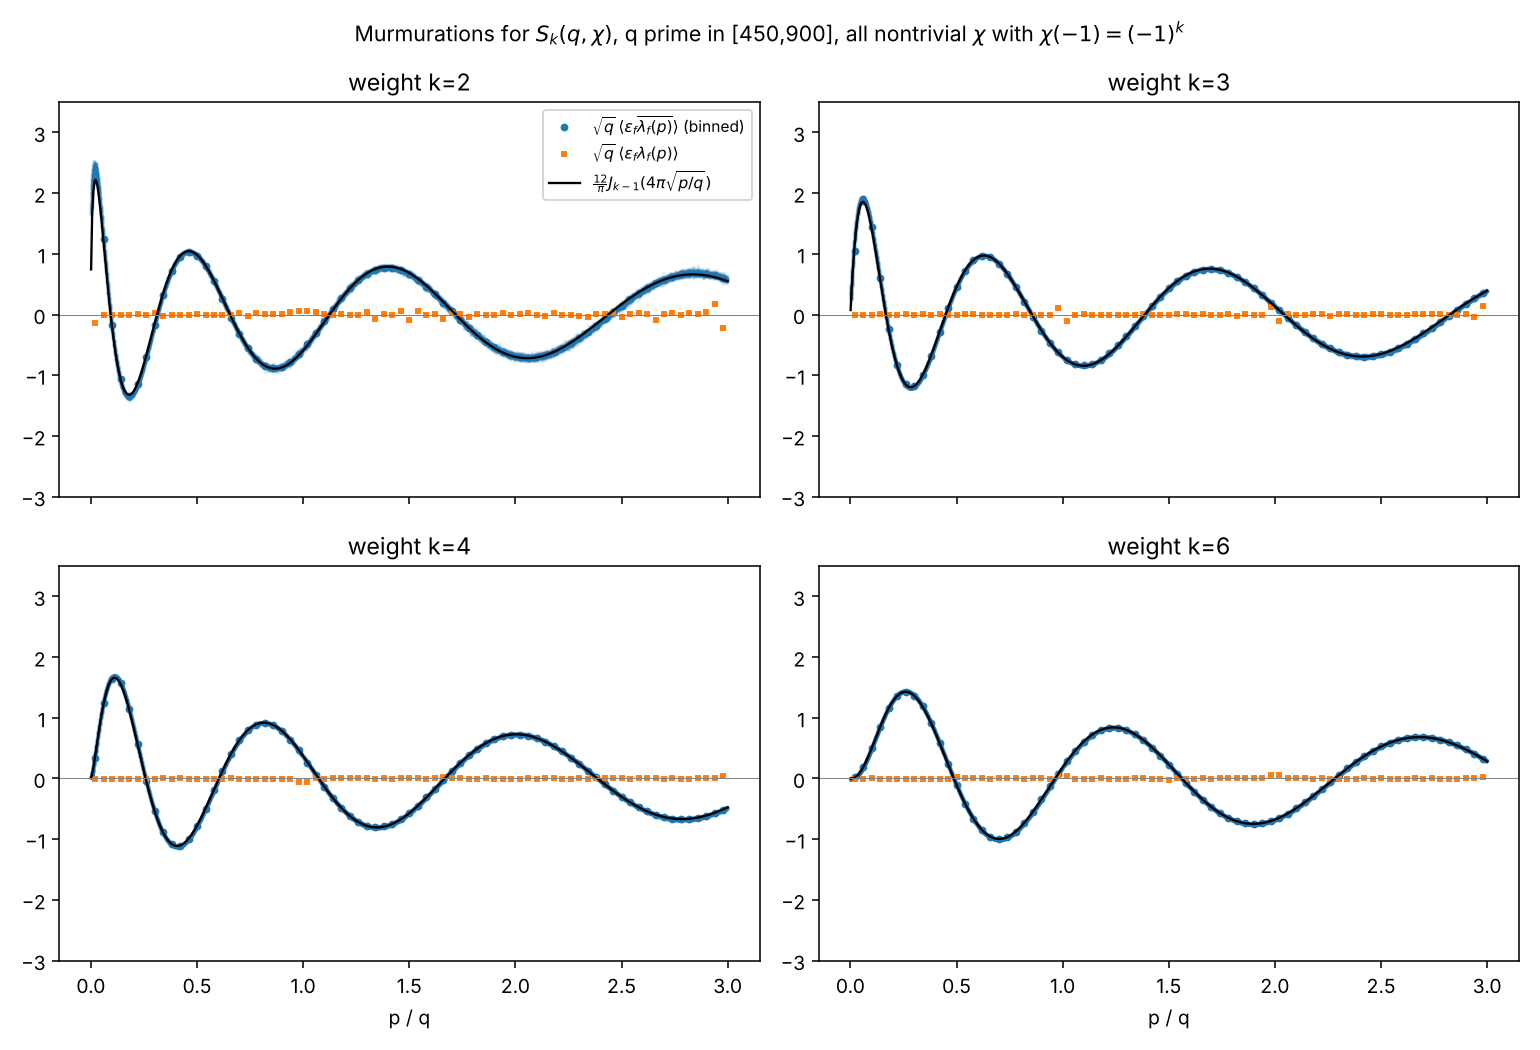
\includegraphics[width=\textwidth]{nebentypus_murmurations.png}
\caption{Blue: $\sqrt q\,\langle\eps_f\ov{\lambda_f(p)}\rangle$ for primes $q\in[450,900]$ (faint dots: individual pairs $(q,p)$; larger dots: bins of width $0.04$). Black: $\frac{12}{\pi}J_{k-1}(4\pi\sqrt{p/q})$. Orange: the unconjugated statistic $\sqrt q\,\langle\eps_f\lambda_f(p)\rangle$.}\label{fig}
\end{figure}

\begin{table}[t]
\centering
\begin{tabular}{rrrrr}
\toprule
$k$ & $p$ & $p/q$ & $\sqrt q\,\langle\eps_f\ov{\lambda_f(p)}\rangle$ & $\frac{12}{\pi}J_{k-1}(4\pi\sqrt{p/q})$\\
\midrule
2 & 79 & 0.099 & $-0.1955$ & $-0.1882$ \\
2 & 397 & 0.498 & $0.9890$ & $0.9882$ \\
2 & 787 & 0.987 & $-0.6187$ & $-0.6398$ \\
2 & 1193 & 1.497 & $0.6727$ & $0.6913$ \\
2 & 1993 & 2.501 & $0.1451$ & $0.1729$ \\
3 & 79 & 0.099 & $1.4597$ & $1.4315$ \\
3 & 397 & 0.498 & $0.4423$ & $0.4416$ \\
3 & 787 & 0.987 & $-0.6575$ & $-0.6554$ \\
3 & 1193 & 1.497 & $0.4266$ & $0.4236$ \\
3 & 1993 & 2.501 & $-0.6577$ & $-0.6481$ \\
4 & 79 & 0.099 & $1.6597$ & $1.6355$ \\
4 & 397 & 0.498 & $-0.7941$ & $-0.7890$ \\
4 & 787 & 0.987 & $0.4208$ & $0.4299$ \\
4 & 1193 & 1.497 & $-0.5740$ & $-0.5811$ \\
4 & 1993 & 2.501 & $-0.3054$ & $-0.3034$ \\
\bottomrule
\end{tabular}
\caption{Natural averages at the single level $q=797$. The last column omits the factor $1+1/p$.}\label{tab}
\end{table}

\begin{table}[t]
\centering
\begin{tabular}{lcccc}
\toprule
 & $q=101$ & $q=211$ & $q=401$ & $q=809$\\
\midrule
$k=2$ (max / mean) & 58.5 / 17.4 & 53.7 / 14.9 & 41.5 / 12.8 & 68.1 / 14.1\\
$k=3$ (max / mean) & 15.2 / 4.9 & 18.7 / 5.0 & 20.0 / 3.9 & 20.5 / 4.7\\
$k=4$ (max / mean) & 17.7 / 3.9 & 16.3 / 4.5 & 18.9 / 3.8 & 16.8 / 4.1\\
\bottomrule
\end{tabular}
\caption{The normalized error $q^{3/2}\,|E(q,p)|$ in Theorem~\ref{thm:natural}, over primes $p<3q$, $p\neq q$.}\label{tab:err}
\end{table}

\section{Squarefree level}\label{sec:composite}

\subsection{Setup and results}
Let $N$ be odd and squarefree, write $\nu(N)=\prod_{\ell\mid N}(\ell+1)$, and let $\cX_k(N)$ be the set of primitive characters $\chi\bmod N$ with $\chi(-1)=(-1)^k$. Each space $S_k(N,\chi)$ with $\chi\in\cX_k(N)$ consists of newforms. We define $\langle\cdot\rangle_h$ and $\langle\cdot\rangle$ as in the introduction, with $q$ replaced by $N$. The analogue of Lemma~\ref{lem:root}, again a consequence of \cite{AL}, is
\begin{equation}\label{eq:rootN}
\eps_f=i^{-k}\,\frac{\tau(\chi)}{\sqrt N}\,\ov{\lambda_f(N)}.
\end{equation}
We verified \eqref{eq:rootN} numerically in all one-dimensional spaces $S_2(21,\chi)$. For this we used our implementation of the trace formula at squarefree level, which we checked independently against Hecke multiplicativity.

\begin{theorem}\label{thm:compositeh}
Let $k\ge2$, let $N$ be odd and squarefree, and let $p\nmid N$ be a prime with $p\le N^2$. Then
\[
\bigl\langle\eps_f\,\ov{\lambda_f(p)}\bigr\rangle_h=\frac{2\pi}{\sqrt N}J_{k-1}\Bigl(4\pi\sqrt{\tfrac pN}\Bigr)+O_{k,\varepsilon}\Bigl(N^{-1+\varepsilon}\bigl(1+\tfrac pN\bigr)^{1/4+\varepsilon}\Bigr).
\]
\end{theorem}

\begin{theorem}\label{thm:compositenat}
Let $k\ge2$, let $N$ be odd and squarefree with $\cX_k(N)\neq\emptyset$, and let $p\nmid N$ be prime. Then
\[
\bigl\langle\eps_f\,\ov{\lambda_f(p)}\bigr\rangle=\frac{2\pi}{\zeta^{(N)}(2)\sqrt N}\Bigl(1+\frac1p\Bigr)J_{k-1}\Bigl(4\pi\sqrt{\tfrac pN}\Bigr)+O_{k,\varepsilon}\Bigl(N^{-1+\varepsilon}\bigl(1+\tfrac pN\bigr)\Bigr),
\]
where $\zeta^{(N)}(2)=\zeta(2)\prod_{\ell\mid N}(1-\ell^{-2})$. Equivalently, the constant $2\pi/\zeta^{(N)}(2)$ equals $\frac{12}{\pi}\prod_{\ell\mid N}\frac{\ell^2}{\ell^2-1}$.
\end{theorem}

The main term in Theorem~\ref{thm:compositenat} dominates for $p\le N^{7/5-\delta}$. For prime $N=q$ the theorem recovers Theorem~\ref{thm:natural}, with a weaker error term. The factor $1/\zeta^{(N)}(2)$ is consistent with Remark~\ref{rem:zeta2}: the character $\bar\chi(n)$ in $L(1,\mathrm{Ad}f)$ restricts the sum to $(n,N)=1$, which gives $\sum_{(n,N)=1}\mu(n)n^{-2}=1/\zeta^{(N)}(2)$. Table~\ref{tab:comp} compares the constant with numerical fits.

\begin{table}[t]
\centering
\begin{tabular}{rlcccc}
\toprule
$N$ & & $\prod_{\ell\mid N}\frac{\ell^2}{\ell^2-1}$ & fit, $k=2$ & fit, $k=3$ & fit, $k=4$\\
\midrule
797 & prime & 1.0000 & 1.0037 & -- & -- \\
471 & $3\cdot157$ & 1.1250 & 1.1409 & 1.1283 & 1.1269\\
687 & $3\cdot229$ & 1.1250 & 1.1347 & 1.1275 & 1.1272\\
865 & $5\cdot173$ & 1.0417 & 1.0496 & 1.0463 & 1.0448\\
851 & $23\cdot37$ & 1.0026 & 1.0176 & 1.0104 & 1.0065\\
899 & $29\cdot31$ & 1.0023 & 1.0153 & 1.0086 & 1.0063\\
\bottomrule
\end{tabular}
\caption{Least-squares fits of $C_N$ in $\langle\eps_f\ov{\lambda_f(p)}\rangle\approx C_N\cdot\frac{12}{\pi\sqrt N}(1+\frac1p)J_{k-1}(4\pi\sqrt{p/N})$ over primes $p<3N$, $p\nmid N$, computed from the exact trace formula, compared with the value $\prod_{\ell\mid N}\ell^2/(\ell^2-1)$ from Theorem~\ref{thm:compositenat}. In a separate test with $N=3\ell$ and $N=5\ell$, $N\le879$, $k=3,4$, the normalized error $N|E|/(1+p/N)$ stays below $3$ and decreases with $N$.}\label{tab:comp}
\end{table}

\subsection{Proof of Theorem \ref{thm:compositeh}}
We follow the proof of Theorem~\ref{thm:main}. For primitive $\chi$ we still have $S_\chi(p,N;N)=\chi(p)\tau(\bar\chi)$ and $\tau(\chi)\tau(\bar\chi)=\chi(-1)N$. So the modulus $c=N$ again contributes exactly $\frac{2\pi}{\sqrt N}J_{k-1}(4\pi\sqrt{p/N})$ for every $\chi$. For the moduli $c=Nr$ with $r\ge2$, write $\chi=\prod_\ell\chi_\ell$. Then $\tau(\chi)=\prod_\ell\chi_\ell(N/\ell)\tau(\chi_\ell)$, which gives
\begin{equation}\label{eq:primsum}
\sum_{\chi\ \mathrm{primitive}}\tau(\chi)\chi(a)=\prod_{\ell\mid N}\Bigl((\ell-1)\,\e\bigl(\overline{a}\,\overline{(N/\ell)}/\ell\bigr)+1\Bigr)\qquad((a,N)=1).
\end{equation}
The parity condition is imposed with the projector $\frac12(1+(-1)^k\chi(-1))$. Expanding the product gives at most $2^{\omega(N)}$ Kloosterman sums of modulus $Nr$, one for each $M\mid N$, with weights $\prod_{\ell\mid M}(\ell-1)\le\varphi(N)$. Since $\overline{(N/M)}\,(N/M)\equiv1\pmod M$, the first argument of the sum indexed by $M$ is $\equiv p(1\pm r)\pmod M$ and $\equiv p\pmod{N/M}$. So its gcd with the modulus divides $(1\pm r,M)$. Weil's bound now applies as before. We also use $\sum_{r\le R}(1\pm r,N)^{1/2}\ll_\varepsilon R\,N^{\varepsilon}$ and $|\cX_k(N)|\gg\varphi(N)\,2^{-\omega(N)}$. \qed

\subsection{Two lemmas for Theorem \ref{thm:compositenat}}
Fix $n=pN$ and let $\psi\bmod N$ be any Dirichlet character, not necessarily primitive. As at prime level, every $s$ with $s^2\mid t^2-4n$ is prime to $N$: if $\ell\mid s$ then $\ell\mid t$, which would force $\ell^2\mid4pN$. The elliptic local factor of the trace formula \cite[Thm.~12.4.11]{CS} is therefore
\[
\sum_{x\bmod N,\ x(x-t)\equiv0}\psi(x)=\psi(t),
\]
including for the principal character $\psi_0$. The Eisenstein term, present only for $K=2$ and $\psi=\psi_0$, is $\sum_{d\mid n,\,(N,n/d)=1}d=N(p+1)$. This gives the following lemma.

\begin{lemma}\label{lem:trN}
For $K\ge2$ and $\psi\bmod N$,
\[
\sum_{t^2<4n}P_K(t,n)\psi(t)H(4n-t^2)=-2\Tr\bigl(T_n\mid S_K(N,\psi)\bigr)+2A_3(\psi)+2N(p+1)\,\delta_{K=2,\,\psi=\psi_0},
\]
where the hyperbolic term satisfies $|A_3(\psi)|\le2^{\omega(N)}\sigma_0(n)\,n^{(K-1)/2}$.
\end{lemma}

\begin{lemma}\label{lem:trbound}
For $K\ge2$ and $\psi=\prod_\ell\psi_\ell\bmod N$,
\[
\bigl|\Tr(T_n\mid S_K(N,\psi))\bigr|\le K\,\sigma_0(p)\,n^{(K-1)/2}\prod_{\ell\mid N,\ \psi_\ell\neq1}(\ell+1)\prod_{\ell\mid N,\ \psi_\ell=1}\Bigl(\frac{\ell+1}{\sqrt\ell}+2\Bigr).
\]
\end{lemma}
\begin{proof}
Decompose $S_K(N,\psi)=\bigoplus_{M}\bigoplus_{d\mid N/M}\{g(dz)\}$, where $g$ runs over the newforms of level $M$ with $\mathrm{cond}(\psi)\mid M\mid N$. The operator $T_n=T_pU_N$ preserves each $2^{\omega(N/M)}$-dimensional oldspace, which is a tensor product of two-dimensional spaces, one for each $\ell\mid N/M$. On this oldspace, $|a_g(p)|\le\sigma_0(p)p^{(K-1)/2}$ by Deligne. For $\ell\mid N/M$ the generalized eigenvalues of $U_\ell$ are the roots of $x^2-a_g(\ell)x+\psi(\ell)\ell^{K-1}$, of modulus $\ell^{(K-1)/2}$. For $\ell\mid M$, we have $|a_g(\ell)|=\ell^{(K-1)/2}$ if $\psi_\ell\ne1$ and $|a_g(\ell)|=\ell^{(K-2)/2}$ if $\psi_\ell=1$ \cite{AL}. Finally, the number of newforms of level $M$ is at most $\dim S_K(M,\psi)\le K\nu(M)$. Summing over $M$ gives the bound, since the resulting sum factors over the primes $\ell\mid N$.
\end{proof}

\subsection{Proof of Theorem \ref{thm:compositenat}}
\emph{The character sum.} By \eqref{eq:primsum}, for $(t,N)=1$,
\[
F(t):=\sum_{\chi\ \mathrm{primitive}}\tau(\chi)\bar\chi(t)=\prod_{\ell\mid N}\bigl((\ell-1)\e(tc_\ell/\ell)+1\bigr)=\e\Bigl(\frac tN\Bigr)\,g(t),
\]
where
\[
g(t)=\prod_{\ell\mid N}\bigl((\ell-1)+\e(-tc_\ell/\ell)\bigr).
\]
and $c_\ell\equiv\overline{N/\ell}\pmod\ell$, so that $\sum_\ell c_\ell/\ell\equiv1/N\pmod1$. We set $F(t)=0$ when $(t,N)>1$. On $(\mathbb Z/\ell)^\times$ we have $\e(x/\ell)=\frac1{\ell-1}\sum_{\psi_\ell}\tau(\bar\psi_\ell)\psi_\ell(x)$, where the sum includes the principal character, whose Gauss sum is $-1$. Hence $g(t)\mathbf 1_{(t,N)=1}=\sum_{\psi\bmod N}B_\psi\psi(t)$ with $B_\psi=\prod_\ell B_{\psi_\ell}$ and
\[
B_{\psi_\ell}=\frac{\ell(\ell-2)}{\ell-1}\quad(\psi_\ell=1),\qquad B_{\psi_\ell}=\frac{\tau(\bar\psi_\ell)\psi_\ell(-c_\ell)}{\ell-1},\quad|B_{\psi_\ell}|=\frac{\sqrt\ell}{\ell-1}\quad(\psi_\ell\ne1).
\]

\emph{An exact formula.} By \eqref{eq:rootN}, Lemma~\ref{lem:trN} with $\psi=\bar\chi$, and the parity projector,
\begin{multline*}
\sum_{\chi\in\cX_k(N)}\sum_f\eps_f\ov{\lambda_f(p)}\\
=\frac{i^{-k}}{\sqrt N\,n^{(k-1)/2}}\Bigl[-\tfrac12\sum_tP_k(t,n)H(4n-t^2)F(t)+\sum_{\chi\in\cX_k(N)}\tau(\chi)A_3(\bar\chi)\Bigr],
\end{multline*}
where we used $\sum_tP_kHF(-t)=(-1)^k\sum_tP_kHF(t)$. After the prefactor, the $A_3$ terms contribute $\ll|\cX_k(N)|\,2^{\omega(N)}\sigma_0(n)\ll N^{1+\varepsilon}$.

\emph{Chebyshev expansion.} With $u_t=t/2\sqrt n$ and $a=4\pi\sqrt{p/N}$ we have $\e(t/N)=\exp(iau_t)$, and Lemma~\ref{lem:cheb} gives
\[
\sum_tP_k(t,n)H(4n-t^2)F(t)=n^{\frac{k-2}2}\sum_{m\ge0}c_m\sum_{\psi\bmod N}B_\psi\sum_tU_m(u_t)\psi(t)H(4n-t^2).
\]
By Lemma~\ref{lem:trN} with $K=m+2$, the inner sum equals $n^{-m/2}\bigl(-2\Tr+2A_3+2N(p+1)\delta_{m=0,\,\psi=\psi_0}\bigr)$. Lemma~\ref{lem:trbound} and the values of $|B_{\psi_\ell}|$ give
\begin{align*}
\sum_\psi|B_\psi|\,n^{-m/2}\bigl(|\Tr|+|A_3|\bigr)&\ll_\varepsilon(m+2)\sqrt n\,N^{\varepsilon}\prod_{\ell\mid N}\Bigl(\tfrac{\ell(\ell-2)}{\ell-1}\bigl(\tfrac{\ell+1}{\sqrt\ell}+2\bigr)+(\ell-2)\tfrac{\sqrt\ell}{\ell-1}(\ell+1)\Bigr)\\
&\ll(m+2)\sqrt n\,N^{3/2+\varepsilon}.
\end{align*}
Combined with $\sum_m(m+2)|c_m|\ll_k(1+a)^2$, this yields
\begin{multline*}
\sum_tP_k(t,n)H(4n-t^2)F(t)\\
=n^{\frac{k-2}2}\Bigl(2c_0N(p+1)\prod_{\ell\mid N}\frac{\ell(\ell-2)}{\ell-1}+O_{k,\varepsilon}\bigl(N^{3/2+\varepsilon}\sqrt n\,(1+p/N)\bigr)\Bigr).
\end{multline*}

\emph{Assembling.} Since $c_0=2i^{k-2}(k-1)J_{k-1}(a)/a$ and $a\sqrt n=4\pi p$, the main term of the numerator is
\[
\frac{(k-1)\sqrt N}{2\pi}\Bigl(1+\frac1p\Bigr)\prod_{\ell\mid N}\frac{\ell(\ell-2)}{\ell-1}\,J_{k-1}(a),
\]
and the error is $O(N^{1+\varepsilon}(1+p/N))$. The denominator is
\[
\sum_{\chi\in\cX_k(N)}\dim S_k(N,\chi)=|\cX_k(N)|\,\frac{(k-1)\nu(N)}{12}\bigl(1+O(N^{-1+\varepsilon})\bigr),\qquad |\cX_k(N)|=\tfrac12\Bigl(\prod_{\ell\mid N}(\ell-2)\pm1\Bigr).
\]
Dividing, and using
\[
\prod_{\ell\mid N}\frac{\ell(\ell-2)}{(\ell-1)(\ell-2)(\ell+1)}=\frac1N\prod_{\ell\mid N}\frac{\ell^2}{\ell^2-1},
\]
completes the proof. \qed

\begin{remark}
At prime level the main term came from the level-one Kronecker--Hurwitz relation. Here it comes from the Eisenstein part of the weight-two trace for the principal character modulo $N$. Its size $2N(p+1)=2\sigma(n)\prod_{\ell\mid N}\frac{\ell}{\ell+1}$ reflects the fact that $\ell$ ramifies in $\mathbb Q(\sqrt{t^2-4pN})$ exactly when $\ell\mid t$. The rest of the constant is the mean value $\ell(\ell-2)/(\ell-1)$ of the local factor $(\ell-1)+\e(-tc_\ell/\ell)$ over $(\mathbb Z/\ell)^\times$.
\end{remark}

\section{Further questions}\label{sec:questions}

We list the questions that the results and numerics suggest most directly. For each one we explain where the difficulty lies and, when we have one, what we expect the answer to be.

\subsection{Secondary terms at prime level}
Table~\ref{tab:err} shows that the error $E(q,p)$ in Theorem~\ref{thm:natural} is of exact order $q^{-3/2}$. Further experiments show that it has structure. We binned $q^{3/2}E(q,p)$ by $y=p/q$ into $15$ intervals of length $0.2$ for $q=401,601,809$. The binned means give the same curve for all three levels: for both $k=2$ and $k=3$, the correlation between the curves for different $q$ is between $0.94$ and $0.97$. The curve has mean close to $0$ and amplitude about $10$--$15$ for $k=2$ and about $5$ for $k=3$. Around it, individual primes $p$ fluctuate by a comparable amount. This suggests an expansion
\[
\bigl\langle\eps_f\,\ov{\lambda_f(p)}\bigr\rangle=\frac{12}{\pi\sqrt q}\Bigl(1+\frac1p\Bigr)J_{k-1}\bigl(4\pi\sqrt y\bigr)+\frac{M_k^{(2)}(y)}{q^{3/2}}+\frac{R_k(q,p)}{q^{3/2}}+o\bigl(q^{-3/2}\bigr),
\]
with a smooth second-order density $M_k^{(2)}$ and an arithmetic fluctuation $R_k(q,p)$ of mean zero.

The terms that the proof of Theorem~\ref{thm:natural} only bounds are natural candidates for $M_k^{(2)}$. These are the values $t\equiv0\pmod q$ excluded in Proposition~\ref{prop:exact}, the Eisenstein term $\delta_{2\mid k}$, the terms $G_k(1)$ and $\min(p,q)^{k-1}G_k(p)$, and the $O(1/q)$ corrections in the normalization. Each of them depends smoothly on $y$. These terms must partly cancel, however. For $k=2$ the Eisenstein term alone would contribute $+24\sqrt y\,q^{-3/2}$, which would give a positive mean that is not observed. The fluctuation $R_k$ presumably comes from the traces $\Tr(T_{pq}\mid S_{m+2}(\SL))$ of the higher Chebyshev modes, which depend on $p$ arithmetically. Determining $M_k^{(2)}$ explicitly, and showing that $R_k$ averages to zero over $p$ in short intervals, would give a two-term asymptotic.

\subsection{From harmonic to natural weights}
Remark~\ref{rem:zeta2} explains the factor $1/\zeta^{(N)}(2)$ through the Petersson formula. A rigorous version would proceed as in \cite{ILS}. Up to local factors at the primes dividing $N$, one writes $\omega_f^{-1}$ in terms of $L(1,\mathrm{Ad}f)$. One approximates $L(1,\mathrm{Ad}f)$ by a short Dirichlet polynomial $\sum_{n\le X}\lambda_f(n^2)\bar\chi(n)n^{-1}$, outside an exceptional set of forms controlled by a zero-density estimate for the adjoint $L$-functions. Then one applies the Petersson formula to each term. The modulus $c=Nn$ should then produce the Ramanujan sum $S(0,N;Nn)=\varphi(N)\mu(n)$, and with it the factor $\sum_{(n,N)=1}\mu(n)n^{-2}$. Such a proof would be less precise than Theorems~\ref{thm:natural} and~\ref{thm:compositenat}. Its advantage is flexibility: it applies whenever the harmonic average can be computed. Examples are $\eps_f\ov{\lambda_f(m)}$ for composite $m$, or smooth averages over $p$, where no analogue of Proposition~\ref{prop:exact} is available.

\subsection{The error term at composite level}
At prime level the error is $O(q^{-3/2+\varepsilon})$, but Theorem~\ref{thm:compositenat} only gives $O(N^{-1+\varepsilon})$. The loss has two sources. The expansion of $g(t)$ into characters has coefficients of size $\sqrt\ell/(\ell-1)$ at each prime. And each trace $\Tr(T_n\mid S_K(N,\psi))$ is bounded individually. The second bound is wasteful. The coefficients $B_\psi$ contain the Gauss sums $\tau(\bar\psi_\ell)$, so by \eqref{eq:rootN} the sum $\sum_\psi B_\psi\Tr(T_n\mid S_K(N,\psi))$ is itself a root-number-weighted average, of the kind studied in this paper, over spaces of lower weight. We expect it to cancel. The numerics support this. For $N=3\ell$ the normalized error $N|E|/(1+p/N)$ falls from $2.7$ at $N=159$ to $0.75$ at $N=879$, which is consistent with a true error of size $N^{-3/2}$. We conjecture that Theorem~\ref{thm:compositenat} holds with error $O(N^{-3/2+\varepsilon}(1+p/N))$.

\subsection{General levels and conductors}
There are two distinct extensions.

\emph{Primitive characters modulo arbitrary $N$.} Atkin and Li \cite{AL} determine the pseudo-eigenvalue at every prime power $\ell^\alpha\parallel N$ at which $\chi$ has full conductor $\ell^\alpha$. We therefore expect \eqref{eq:rootN} to hold whenever $\chi$ is primitive modulo $N$, for $N\not\equiv2\pmod4$. The main term in the proof of Theorem~\ref{thm:compositeh} uses only primitivity and $\tau(\chi)\tau(\bar\chi)=\chi(-1)N$, so the harmonic result should extend with little change. The natural result needs more work. When $\ell^2\mid N$, conductor indices divisible by $\ell$ appear in the trace formula, and the elliptic local factors are no longer simply $\psi(t)$.

\emph{Characters of smaller conductor.} If $\mathrm{cond}(\chi)<N$, then $S_k(N,\chi)$ contains oldforms. These must be removed, for instance by inverting the trace formula over divisors of $N$. A more serious problem appears at primes with $\ell^2\mid N$ where $\chi_\ell$ is not of full conductor. There the local representation can be supercuspidal or a ramified principal series, $a_f(\ell)$ can vanish, and Lemma~\ref{lem:root} has no analogue. The local root numbers are then epsilon factors of the local representations, and averaging over them resembles the depth aspect of \cite{Tom}. It would be interesting to understand how the average over characters studied here interacts with the averaging over local representations in \cite{Tom}.

\subsection{Characters of fixed order}
For a single character the proof of Theorem~\ref{thm:main} gives an exact formula. Let $\chi\in\cX_k(q)$ and $(r,q)=1$. Twisted multiplicativity of Kloosterman sums, together with $\sum_d\chi(d)\e(a\bar d/q)=\chi(a)\tau(\bar\chi)$, gives
\[
S_\chi(p,q;qr)=\chi(p\bar r)\,\tau(\bar\chi)\,S(p\bar q,1;r).
\]
We checked this identity numerically. Inserting it into \eqref{eq:pet}, the Gauss sums cancel exactly, and
\begin{equation}\label{eq:single}
\sum_{f\in\cB_k(q,\chi)}\omega_f\,\eps_f\ov{\lambda_f(p)}=\frac{2\pi}{\sqrt q}\sum_{\substack{r\ge1\\(r,q)=1}}\bar\chi(r)\,\frac{S(p\bar q,1;r)}{r}\,J_{k-1}\Bigl(\frac{4\pi}{r}\sqrt{\frac pq}\Bigr)+\bigl(\text{terms with }q\mid r\bigr).
\end{equation}
In this language Theorem~\ref{thm:main} says that the average of $\bar\chi(r)$ over $\cX_k(q)$ kills every $r\not\equiv\pm1\pmod q$, so only $r=1$ survives.

For a single character the terms $r\ge2$ in \eqref{eq:single} are as large as the term $r=1$. Consider therefore families of characters of a fixed order $d$, averaged over prime levels $q\equiv1\pmod d$ with $p/q\approx y$. We expect a density of the form
\[
2\pi J_{k-1}(4\pi\sqrt y)+2\pi\sum_{r\ge2}\frac{\kappa_d(r;p)}{r}\,J_{k-1}\bigl(4\pi\sqrt y/r\bigr),
\]
where $\kappa_d(r;p)$ is the average of $\bar\chi_q(r)S(p\bar q,1;r)$ over the family.

\emph{Quadratic $\chi$.} Here the individual forms are still not self-dual. The relation $\ov{a_f(p)}=\chi(p)a_f(p)$ shows that $\bar f=f\otimes\chi$, which is in general a different form; only the space $S_k(q,\chi)$ is closed under $f\mapsto\bar f$. By quadratic reciprocity, $\chi_q(r)=(r/q)$ depends only on $q\bmod4r$. The Kloosterman sum $S(p\bar q,1;r)$ depends only on $p$ and $q$ modulo $r$. So $\kappa_2(r;p)$ is an explicit local density, which can be computed from the distribution of primes $q$ in residue classes modulo $4r$, and it depends on $p\bmod r$. The resulting murmuration density is genuinely arithmetic, and it fluctuates with $p$ even after scaling.

\emph{Cubic $\chi$.} Similarly, $\chi_q(r)$ is a cubic residue symbol, and cubic reciprocity in $\mathbb Z[\omega]$ expresses its average in terms of residue classes of primary primes. Because the Gauss sums cancel in \eqref{eq:single}, no information on the distribution of cubic Gauss sums is needed.

Computing $\kappa_d$ explicitly, and comparing the resulting densities with Zubrilina's for trivial character, seems a natural next step.

\subsection{Beyond the Petersson range}
For $p\asymp N^2$ the argument of $J_{k-1}(4\pi\sqrt{p/N}/r)$ is $\asymp\sqrt N/r$, and all moduli $c=Nr$ with $r\ll\sqrt N$ contribute at comparable size, so the range $p\le N^{2}$ in Theorem~\ref{thm:compositeh} cannot be extended by this method. The main terms of Theorems~\ref{thm:natural} and~\ref{thm:compositenat} also stop dominating, at $p\asymp q^{9/5}$ and $p\asymp N^{7/5}$ respectively. What is the true size of $\langle\eps_f\ov{\lambda_f(p)}\rangle$ for $N^2\le p\le N^{3}$? A natural guess is square-root cancellation over the family, which has about $N^2$ members, giving size about $N^{-1}$. This would mean that the Bessel law stops at $p\asymp N^2$. Cardi \cite{Car} finds a pointwise range of cubic size for trivial character, which suggests checking whether an analogous threshold exists here.

\subsection{Other families and statistics}
\emph{Maass forms with nebentypus.} The Kuznetsov formula has the same Kloosterman sums $S_\chi(m,n;c)$ as \eqref{eq:pet}. So the cancellation at the modulus $c=N$ should give a main term equal to the Kuznetsov transform of the test function, evaluated at $4\pi\sqrt{p/N}$, at each level. Lowry-Duda \cite{LD} points out obstacles to Maass murmurations at general level with existing methods. Averaging over characters may avoid some of them.

\emph{Low-lying zeros.} Murmurations are closely related to lower-order terms in the one-level density of low-lying zeros, through the explicit formula. For the non-self-dual families studied here one expects unitary symmetry. Because the correlation between $\eps_f$ and $\ov{\lambda_f(p)}$ is so simple, it may be possible to compute the lower-order terms of the one-level density of these families explicitly.

\begin{thebibliography}{99}
\bibitem{AL} A.~O.~L.~Atkin and W.-C.~W.~Li, Twists of newforms and pseudo-eigenvalues of $W$-operators, \emph{Invent. Math.} \textbf{48} (1978), 221--243.
\bibitem{BBLLD} J.~Bober, A.~R.~Booker, M.~Lee and D.~Lowry-Duda, Murmurations of modular forms in the weight aspect, \emph{Algebra Number Theory} \textbf{20} (2026), 299--332.
\bibitem{BLLDSHZ} A.~R.~Booker, M.~Lee, D.~Lowry-Duda, A.~Seymour-Howell and N.~Zubrilina, Murmurations of Maass forms, arXiv:2409.00765.
\bibitem{Car} J.~Cardi, Joint level-weight murmurations: prime averaging and the cubic pointwise range, arXiv:2607.08982.
\bibitem{CS} H.~Cohen and F.~Str\"omberg, \emph{Modular Forms: A Classical Approach}, Graduate Studies in Mathematics 179, Amer. Math. Soc., 2017.
\bibitem{Cow} A.~Cowan, Murmurations and ratios conjectures, arXiv:2408.12723.
\bibitem{HLOP} Y.-H.~He, K.-H.~Lee, T.~Oliver and A.~Pozdnyakov, Murmurations of elliptic curves, \emph{Exp. Math.}
\bibitem{ILS} H.~Iwaniec, W.~Luo and P.~Sarnak, Low lying zeros of families of $L$-functions, \emph{Publ. Math. IH\'ES} \textbf{91} (2000), 55--131.
\bibitem{IK} H.~Iwaniec and E.~Kowalski, \emph{Analytic Number Theory}, Amer. Math. Soc. Colloquium Publications 53, 2004.
\bibitem{KL} C.~I.~Kuan and D.~Lesesvre, Murmurations using Petersson trace formula, arXiv:2507.11418.
\bibitem{LD} D.~Lowry-Duda, On murmurations and trace formulas, arXiv:2506.01640.
\bibitem{LOP} K.-H.~Lee, T.~Oliver and A.~Pozdnyakov, Murmurations of Dirichlet characters, \emph{Int. Math. Res. Not. IMRN}.
\bibitem{Tom} L.~Tomczak, Murmurations in the depth aspect for Maass and modular forms, arXiv:2606.08353.
\bibitem{Wat} G.~N.~Watson, \emph{A Treatise on the Theory of Bessel Functions}, 2nd ed., Cambridge University Press, 1944.
\bibitem{Zub} N.~Zubrilina, Murmurations, \emph{Invent. Math.} (2025).
\end{thebibliography}

\end{document}
